\chapter{Mobile Autonomous Shotcrete and Scanning System Overview}
\label{chap:overview}
\section{Hardware}
\subsection{Husky}
%https://www.clearpathrobotics.com/husky-unmanned-ground-vehicle-robot/
Clearpath Robotics's Husky Unmanned Ground Vehicle (Husky UGV) shown in Figure \ref{fig:husky} is the mobile base used for the proof-of-concept prototype. It is a four wheeled skid steer vehicle, capable of driving on uneven ground or loose gravel. It has a wheel diameter of 330 mm, and external dimensions of 990 mm $\times$ 670 mm $\times$ 390 mm. Its maximum payload is 75 kg and has a maximum speed is 1.0 m/s. Skid steer vehicles have notoriously unreliable odometry data which makes the Husky an excellent choice as a mobile base, since it creates a more realistic representation of the final product.\\
\begin{figure}[H]
    \centering
    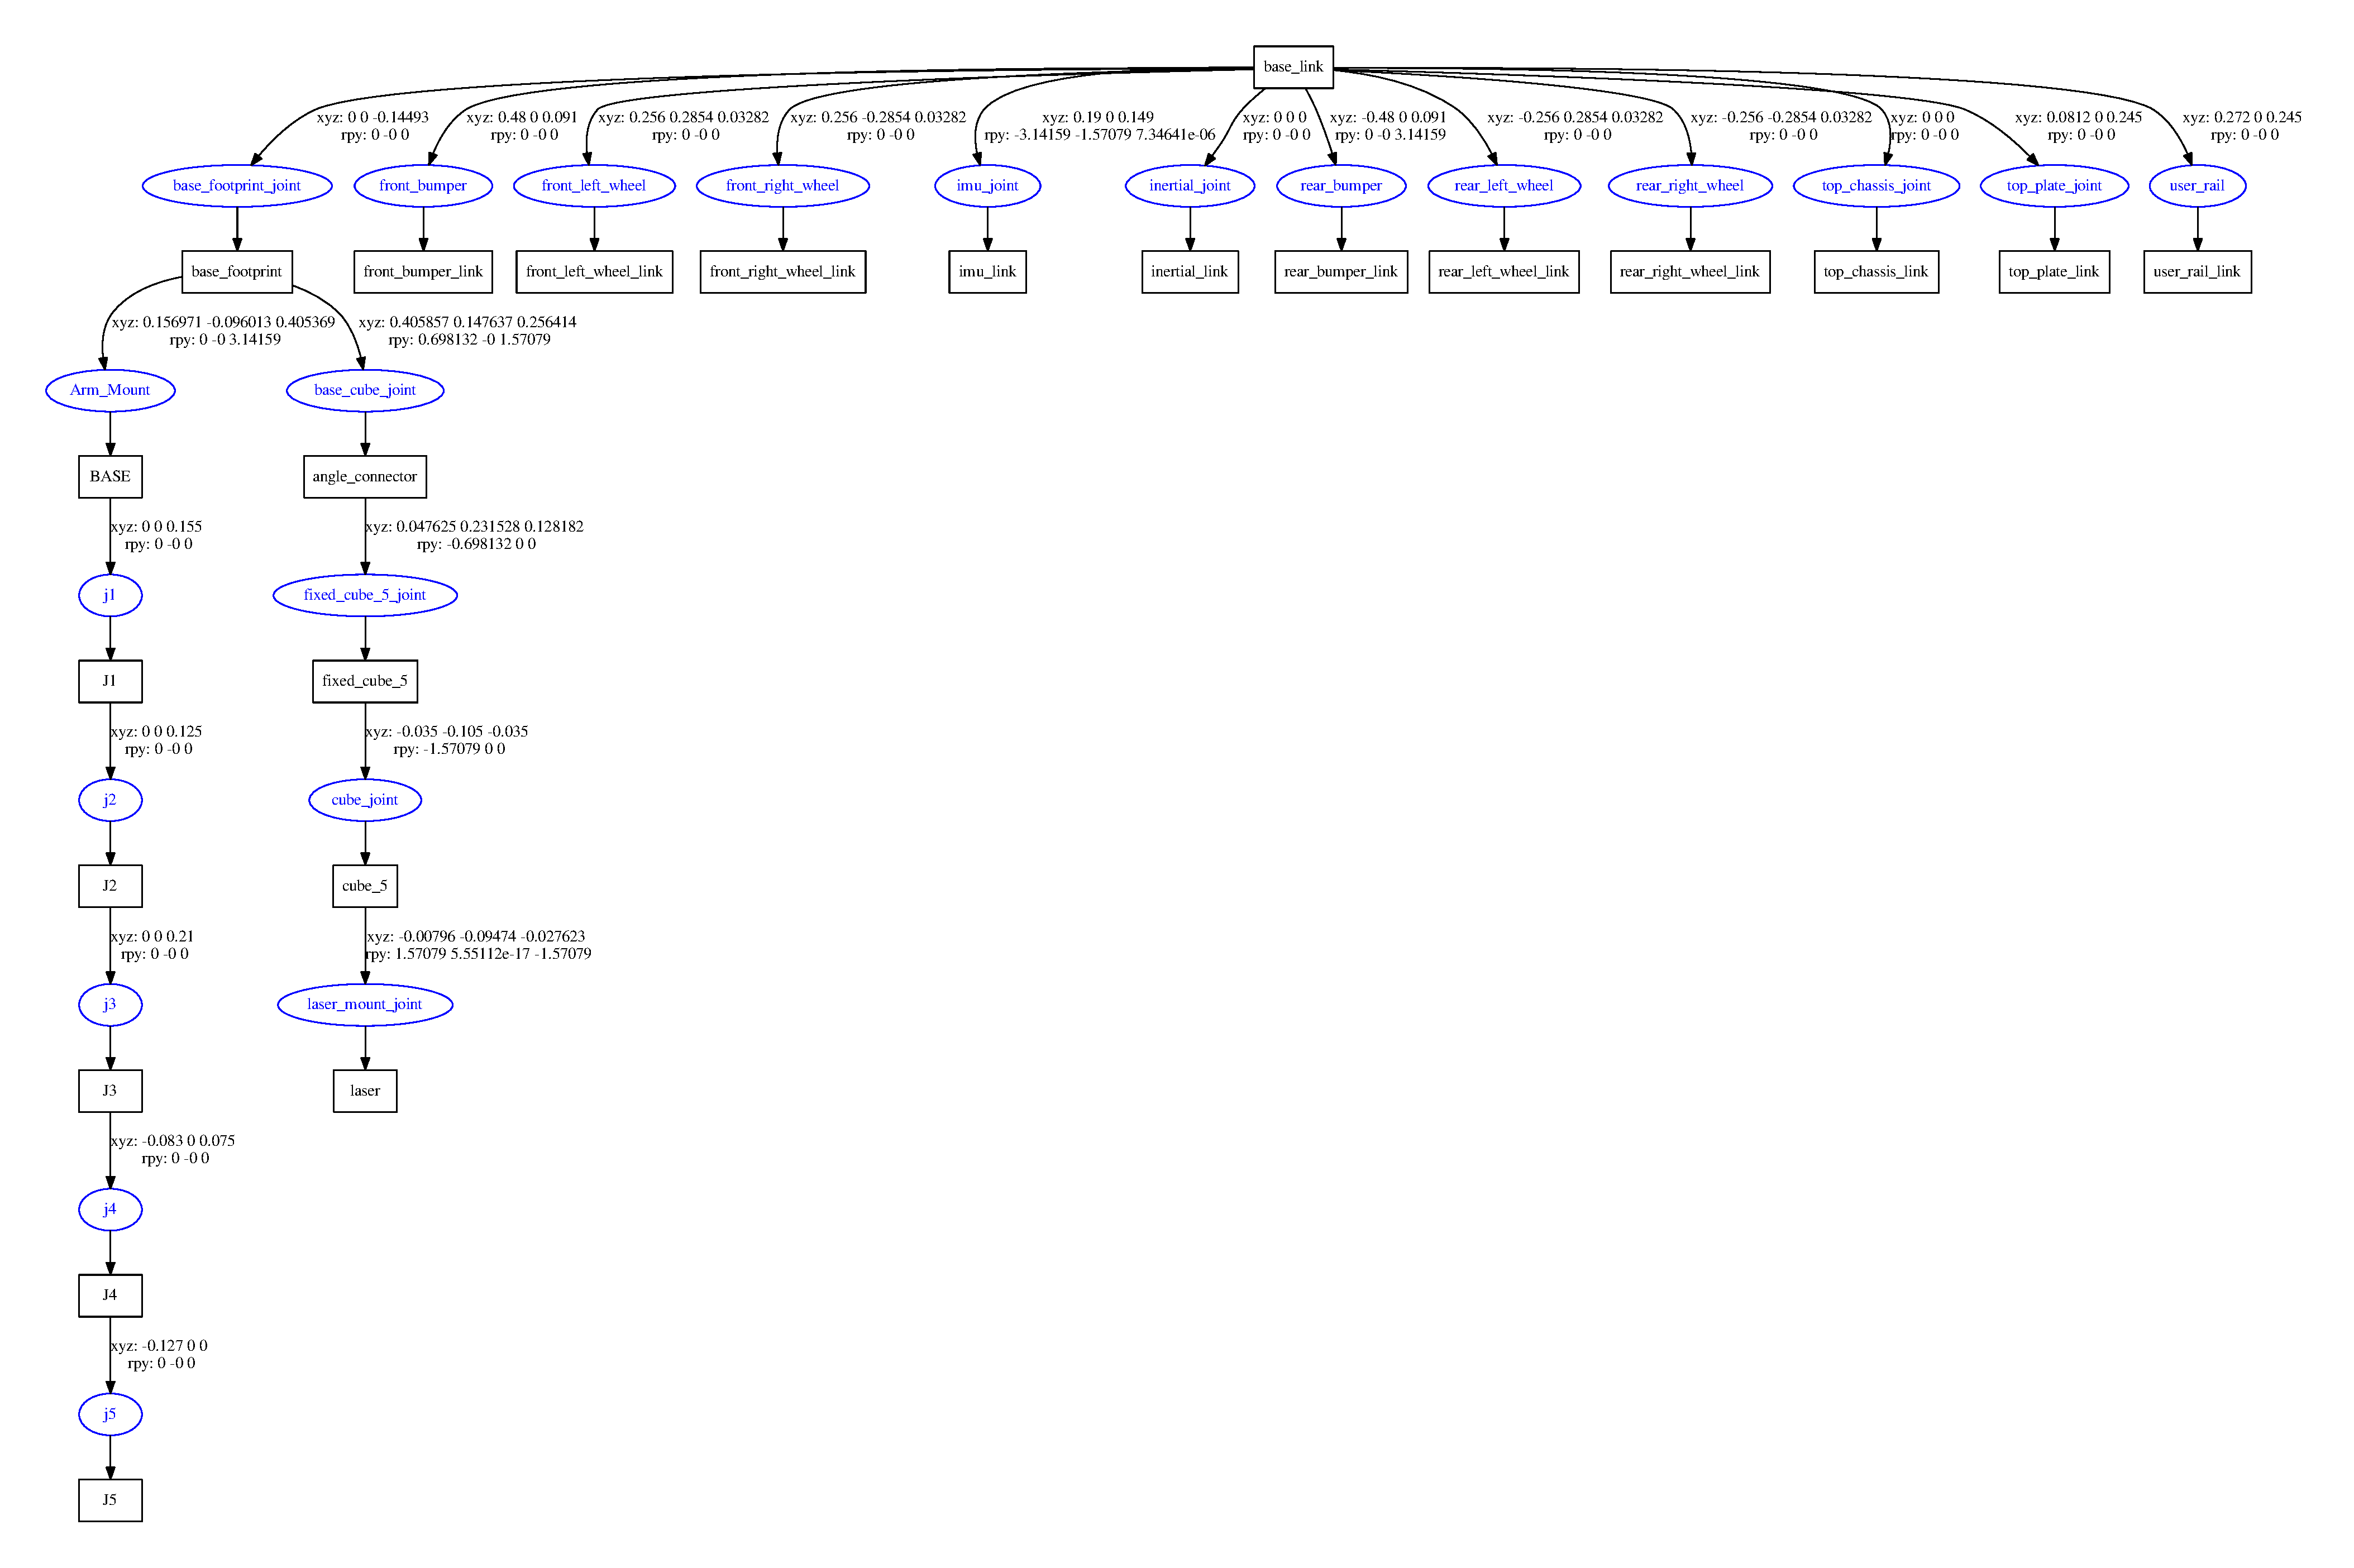
\includegraphics[width=0.8\textwidth]{Pics/husky.jpg}
    \caption{Husky UGV \cite{huskypage}}
    \label{fig:husky}
\end{figure}
\subsection{Husky Peripherals}

\begin{figure}[htb]
    \centering
    \includegraphics[width=\textwidth]{Pics/DSC0433.JPG}
    \caption{Husky with Peripherals Attached}
    \label{fig:peripherals}
\end{figure}
The Husky required a few modifications to support the additional hardware used. A top plate was machined to mount the manipulator as well as a mounting bracket for the nodding head servo. A trailer hitch was installed and a trailer was built to allow the Husky to tow additional batteries, a generator, and the controller for the manipulator.\\
\subsection{DENSO VP6242}
\begin{figure}[H]
    \centering
    \includegraphics[width=0.6\textwidth]{Pics/denso.png}
    \caption{DENSO VP6242 Manipulator \cite{densopage}}
    \label{fig:densofig}
\end{figure}
%https://www.denso-wave.com/en/robot/product/five-six/vp.html
The final product will likely use hydraulics to position the shotcreting and scanning end-effector. Since the payload and forces will require a high strength and rigidity manipulator, using electric motors would be infeasible. Designing a manipulator for this task is outside the scope of this research, so a suitable analogue was chosen. The requirements of the manipulator is that it can position its end-effector with 6 degrees-of-freedom like the final version, but does not require the same workspace, strength, or rigidity the final product would in order to accurately position the end-effector and apply shotcrete. The DENSO manipulator shown in Figure \ref{fig:densofig} was chosen since it fulfils all the application requirements and was available at \acrshort{uoit} for use in this work. It has a maximum reach of 432 mm and a maximum payload of 2.5 kg.\\ 
\subsection{LMS101}

\begin{figure}[H]
    \centering
    \includegraphics[width=0.25\textwidth]{Pics/sick.png}
    \caption{SICK LMS101 \acrshort{lidar} \cite{sickpage}}
    \label{fig:sick}
\end{figure}
%https://www.sick.com/de/en/detection-and-ranging-solutions/2d-\acrshort{lidar}-sensors/lms1xx/lms101-10000/p/p346868?ff_data=JmZmX2lkPXAzNDY4NjgmZmZfbWFzdGVySWQ9cDM0Njg2OCZmZl90aXRsZT1MTVMxMDEtMTAwMDAmZmZfcXVlcnk9JmZmX3Bvcz04JmZmX29yaWdQb3M9OCZmZl9wYWdlPTEmZmZfcGFnZVNpemU9OCZmZl9vcmlnUGFnZVNpemU9OCZmZl9zaW1pPTkzLjA=
The LMS101 shown in Figure \ref{fig:sick} is a \acrshort{lidar} scanner manufactured by SICK. It has an aperture angle of 270$\degree$, angular resolution of 0.25$\degree$ at 25 Hz, and optimal range of 0.5 m - 20 m. SICK is a well know brand of \acrshort{lidar} scanners, with lots of software drivers available for the various systems it works with. The \acrshort{ros} driver for this \acrshort{lidar} does not natively support 0.25$\degree$ resolution, so it has been modified accordingly for this work. It has a systematic error of $\pm$30 mm and statistical error of 12 mm, though through testing it was found the \acrshort{lidar} performs much better in the given test conditions. With an Ingress Protection (\acrshort{ip}) rating of \acrshort{ip}65, it is suitable for indoor use but can be replaced with another model from the same family with equal performance but higher \acrshort{ip} rating (up to \acrshort{ip}67).\\
\subsection{Schunk Powercube PR70}
\begin{figure}[H]
    \centering
    \includegraphics[width=0.27\textwidth]{Pics/powercube.png}
    \caption{Schunk Powercube PR70 \cite{schunkpage}}
    \label{fig:schunk}
\end{figure}
The \acrshort{lidar} used must be mounted on a nodding head to generate 3D point clouds. The Powercube PR70 made by Schunk was chosen for this task partly since it was already an asset of the \acrshort{uoit} \acrshort{mars} Lab and can be seen in Figure \ref{fig:schunk}. The module has higher accuracy and payload than the application requires, but since it was an unused asset it was chosen for this application for practicality reasons. It has a nominal torque of 15 Nm, repeat accuracy of 0.03$\degree$, maximum angular velocity of 240$\degree$/s, and maximum acceleration of 960$\degree$/s$^2$. The Powercube PR70 can be seen mounted on the MASS with the LMS101 \acrshort{lidar} attached in Figure \ref{fig:lidarmass}.\\
\begin{figure}[H]
    \centering
    \includegraphics[width=0.67\textwidth]{Pics/zoom.jpg}
    \caption{MASS Nodding Head Assembly}
    \label{fig:lidarmass}
\end{figure}
\section{Open Source Software}
\label{sec:software}
All software integrated and developed for this research is intended for use within the \acrshort{ros} framework. Since \acrshort{ros} is an open source community with many packages available for use in research, it offers a wide selection of resources useful to this work.\\

Many of the tasks required for operation of the MASS have already been developed by the \acrshort{ros} community. Hardware drivers, motion controllers, \acrshort{lidar} scan to point cloud assemblers, navigation, and mapping packages are already available for use through \acrshort{ros} and the open source licenses they contain. The following open source packages were implemented on the MASS.\\
\subsection{RViz}
\label{sec:RViz}

Complete documentation on RViz can be found at \url{http://wiki.ros.org/RViz}\\

RViz is a powerful visualization tool developed for use with \acrshort{ros}. There is a large quantity of information that can be generated using \acrshort{ros} that is not easily interpreted without the use of an interactive graphical user interface. RViz allows users to view, interact with, interpret, and modify the data handled within \acrshort{ros}. RViz is an invaluable tool in mobile robotics: it can display a model of the robot, a map the robot has generated of its environment, the path it intends to follow, and display sensor data the robot acquires. The user can interact with RViz and send commands to the robot such as: position goals, movement commands, status changes, or selecting parts of the sensor data to be used in other software algorithms.\\

RViz is designed to be adaptable for whatever the operator needs. Custom tools and plugins are easily developed to make RViz helpful in the context it is used. In this work, a custom tool was implemented for selecting sections of the mine surface to be scanned or shotcreted. A custom plugin called the control panel was created to provide a user-friendly interface to command and control all relevant aspects of the MASS.\\

RViz configurations can be saved to a file and loaded at launch when the robot control system is brought online. The configuration file for this work sets the RViz environment in a way that is practical for the operator, but includes options to reveal information useful for debugging and research. For example, under most circumstances the point cloud representation of the mine surface should be shown but individual laser scans hidden. If the operator wanted to see the instantaneous view of the robot's environment represented as a laser scan, the topic's checkbox simply needs to be checked. When generating trajectories the surface path, surface normals, and end-effector path are shown, however, the operator may only want some or none of the information displayed so they are all easily hidden or shown. This is all accomplished through the ``Displays'' panel of RViz. The configuration file subscribes RViz to all the relevant topics and automatically hides the topics containing information that does not need to be displayed.\\

\subsection{Husky}

Complete documentation of the Husky package can be found at \url{http://wiki.ros.org/Robots/Husky}\\

The Husky package is made by Clearpath Robotics to provide \acrshort{ros} functionality to their Husky Unmanned Ground Vehicle (UGV). The package consists of the following subpackages:

\begin{itemize}
    \item \node{husky_base}
    \item \node{husky_bringup}
    \item \node{husky_gazebo}
    \item \node{husky_viz}
    \item \node{husky_control}
    \item \node{husky_description}
    \item \node{husky_msgs}
    \item \node{husky_navigation}
\end{itemize}

\paragraph{husky\_base}

The \node{husky_base} package provides the low level communication between \acrshort{ros} and the robot. It contains all the necessary drivers to allow the robot to operate under \acrshort{ros} control.\\

\paragraph{husky\_bringup}

The \node{husky_bringup} package contains a number of scripts to that launch all the necessary packages (like \node{husky_base}) for the robot to function. Many applications for the Husky robot are intended to be turnkey, so the bringup package allows the designer to set what packages to launch when the robot boots up. Using the bringup package the robot can be configured to commence its control system as soon as it is powered on.\\

\paragraph{husky\_gazebo}

Gazebo is a simulation tool used in \acrshort{ros}. With a fully defined robot model, Gazebo can simulate the robot in a user defined environment. If an operator intends to test their algorithms on a Husky robot, but does not have access to a physical robot they can test their software on a simulated version of the Husky. Similarly, if the operator wants to test their robot in a scenario that may cause damage to the robot or in an environment they are unable to create, they can use Gazebo to test their algorithms in simulation.\\

\paragraph{husky\_viz}

RViz configurations can be saved and loaded by \acrshort{ros}. The \node{husky_viz} package contains various configurations for RViz that optimize its configuration for use with the Husky.\\

\paragraph{husky\_control}

The package \node{husky_control} turns motion goals into actual robot motion. The motion goals are published using \acrshort{ros} topics and the \node{husky_control} package subscribes to these topics and moves the robot accordingly. The motion goals can be provided directly from the operator using an input device such as a joystick or generated from autonomous navigation packages acting on a goal location provided by the operator. The source of the motion commands does not affect how the package functions, so it is able to receive motion commands from a wide variety of sources as long as the commands are formatted using the appropriate \acrshort{ros} message type.\\ 

\paragraph{husky\_description}

In order to visualize the robot in the RViz environment, the robot requires a description. The robot description contains all the relevant information about the robot parts, which way they can move, what material they are, and how to visually represent them. The description also contains the relevant physical characteristics to simulate the robot in Gazebo. The \node{husky_description} package uses the Unified Robot Description Format (\acrshort{urdf}) to describe the model for the Husky UGV.\\

\paragraph{husky\_msgs}

To communicate with other packages, or within the Husky packages, custom messages for the Husky robot are used. The \node{husky_msgs} package contains these custom messages. An example of the HuskyStatus message can be found in Appendix \ref{app:huskystatus}

%\includecode[pythonstyle]{Code/HuskyStatus.msg}{HuskyStatus.msg}

\paragraph{husky\_navigation}

The \node{husky_navigation} package provides configurations and examples for using varous navigation packages with the Husky. It contains all the relevant information a navigation package requires to successfuly apply the navigation algorithm on the Husky. Parameters such as the robot's footprint size, how far away to stay from obstacles, what sort of behaviours to exhibit when encountering obstacles, and what sensor information is available are contained within the configuration files. Navigation packages configure their global and local planners with the files contained in the \node{husky_navigation} package. The configuration file for producing costmaps for use in navigation is shown in Appendix \ref{app:huskyconfig} . The package contains launch files to use various navigation packages with the Husky robot as well as demos that will launch the required accompanying packages. Launch files for \acrshort{amcl}, GMapping, Frontier Exploration, and Move Base packages are included as well as an empty map for use when the robot is being simulated in Gazebo.\\ 
\clearpage
\subsection{Move Base}

Complete documentation of the Move Base package can be found at \url{http://wiki.ros.org/move_base}\\

\begin{figure}[H]
    \centering
    \includegraphics[width=\textwidth]{Pics/overview_tf.png}
    \caption{Overview of the Move Base Package \cite{rosmovebase}}
    \label{fig:movebaseoverview}
\end{figure}

The \node{move_base} package takes high level commands such as a location goal and performs the necessary actions to drive the robot to that location. A graphical overview of the package is shown in Figure \ref{fig:movebaseoverview}. It divides the task among two planners, the global planner and the local planner. The global planner is responsible for creating the overall plan for the robot path. It uses a global costmap generated by the map server, which holds the map generated by the \acrshort{slam} algorithm or loaded from file. The global costmap includes things like the inflation layer, which acts as a safety buffer by creating a region surrounding any obstacles within the map that the robot cannot enter. The local costmap is generated based on what the robot's sensors currently detect. If a person were to walk in front of the robot they would appear in the local costmap and the local planner would generate a path around the obstacle, attempting to return to the path generated by the global planner. If a person or object is placed close enough to the robot such that the robot is now within the inflation layer of the obstacle, it is considered stuck. Once stuck, the robot must execute recovery behaviours to become unstuck. Figure \ref{fig:recovery} shows what recovery behaviours \node{move_base} uses to free itself. First the robot deletes obstacles from the map that are further away than a user specified distance. If the robot is then free to move, it will continue its navigation. If the robot is still stuck, it will rotate on the spot to get an updated view of its surroundings. If it still cannot move it will clear the map of all obstacles that are not within the area it needs to rotate in place. If it is still stuck, it will rotate once more to scan its environment for obstacles. Once the second clearing rotation is complete, if it is still unable to move, it will abort its current goal and release a message notifying the system it was unable to reach its target location.\\

\begin{figure}[H]
    \centering
    \includegraphics[width=\textwidth]{Pics/recovery_behaviors.png}
    \caption{Move Base Recovery Behaviours \cite{rosmovebase}}
    \label{fig:recovery}
\end{figure}

\subsection{Laser Assembler}


Complete documentation of the Laser Assembler package can be found at \url{http://wiki.ros.org/laser_assembler}\\

The \node{laser_assembler} package converts the stream of laser scan data to a point cloud. When the MASS creates a point cloud representation of its surroundings, it tells the \node{laser_assembler} package when to start and stop recording the laser scans generated by the LMS101 \acrshort{lidar} scanner. The assembler will store all of the laser scans, along with the coordinate frame transformation from a fixed frame to the \acrshort{lidar} frame at that moment. When the point cloud scan is complete, \node{laser_assembler} is notified and produces a point cloud in the coordinate frame requested by the user. Discussed further in Section \ref{sec:locsourceerror}, the parameter \var{ignore_laser_skew} can be set so that each point in the laser scan is transformed using the current pose of the \acrshort{lidar} rather than transforming the whole scan at once. Accuracy can be improved if the position of the nodding head is updated more than once during the time it takes to perform a single point cloud scan.\\

\subsection{Hector SLAM}

Complete documentation of the Hector \acrshort{slam} package can be found at \url{http://wiki.ros.org/hector_slam}\\

The \node{hector_slam} package contains the \node{hector_mapping} package used by the MASS to perform \acrshort{slam}. The two main \acrshort{slam} packages available for use with \acrshort{ros} are GMapping and Hector \acrshort{slam}. GMapping is a more popular algorithm, but requires odometry from the robot. Hector \acrshort{slam} can perform \acrshort{slam} without the need for odometry. While the MASS does measure its odometry, it is intended for use on uneven rocky ground and odometry may not be reliable. For that reason, Hector \acrshort{slam} was chosen as the \acrshort{slam} algorithm for use on the MASS. However, thanks to the modularity that \acrshort{ros} offers, it is a simple task to utilize other \acrshort{slam} algorithms like GMapping on the MASS.\\

\subsection{RQT Reconfigure}

Complete documentation of the RQT Reconfigure package can be found at \url{http://wiki.ros.org/rqt_reconfigure}\\

If a node has been configured with parameters that can change at runtime, \node{rqt_reconfigure} can be used to modify them. When the user launches the Graphical User Interface (\acrshort{gui}), it will poll the \acrshort{ros} parameter server to determine which nodes have dynamically reconfigurable variables and what their values and acceptable ranges are. It then presents the user with a window that shows a list of nodes on the left. When a node is selected, the configurable parameters are shown on the right, most often in the form of a slider bar. An example \node{rqt_reconfigure} \acrshort{gui} window can be seen in Figure \ref{fig:dyngui2}.

\begin{figure}[h]
    \centering
    \includegraphics[width=\textwidth]{Pics/dyngui.png}
    \caption{\texttt{rqt\_reconfigure} \acrshort{gui}}
    \label{fig:dyngui2}
\end{figure}

\section{Software Contributions}
\label{sub:software}

A thorough discussion of the source code is provided in Appendix \ref{app:code} with the complete code given in Appendix \ref{app:code}. The following table of contents outlines the software contributons of this work:

\begin{minipage}{\textwidth}

\end{minipage}

The main interface between the user and the control system occurs within an RViz window. Along with the regular features of RViz, this software adds a panel and a tool to the RViz interface. The additional features can be seen in Figure \ref{fig:panel} labeled as Control Panel (right) and Selection Tool (top). The code for the control panel is split between two files. For the system's current purpose, it would be far less functional to have a standalone \acrshort{gui} and not use RViz for visualization. Therefore, \node{control_dashboard} was designed as a plugin for RViz. As future work on this project continues, the need for RViz visualization may diminish, so the node was designed to make converting it to run without RViz a trivial task. Eventually, when this system is implemented in a mine, no graphical interface at all will be required on the machine itself. For that reason, the core functionality of the system lies in the \node{control_panel} node. The \node{control_dashboard} node simply relays the actions from the user interface to the \node{control_panel} node.\\

\begin{figure}[ht!]
    \centering
    \includegraphics[width=.7\textwidth]{Pics/guidrawing.pdf}
    \caption{MASS \acrshort{gui} Panel}
    \label{fig:thegui}
\end{figure}

The \node{control_panel} node is the heart of the control system. It is responsible for calling the localization, trajectory generation, and thickness estimation services, as well as communication with the DENSO arm, Powercube servo, and Husky UGV. Other MASS-specific requirements such as cropping regions from the robots perception that are occupied by the robot itself or  modifying trajectory points to fit within the DENSO arm's workspace are performed by the \node{control_panel} node. \\

The main contribution of this work to the \acrshort{ros} community are the localization, trajectory generation, and thickness estimation services. These three services are intended to be as portable as possible so they can be useful in any robotics project, regardless of the system configuration. Should other researchers have a need for the service they provide, one simply needs to install the package and they will be able to launch the desired service from the terminal or their own launch file. Unfortunately, due to this document's confidentiality, the source code will not be made available, so the functionality of the compiled binaries are provided as-is. Any of the parameters that can be modified by the user are still accessible, but the source code cannot be viewed or modified.\\
\subsection{User Interface}
\label{sub:gui}
\begin{figure}[H]
    \centering
    \includegraphics[width=\textwidth]{Pics/sixpt9.png}
    \caption{RViz User Interface}
    \label{fig:panel}
\end{figure}
%%%%%%%%%%%%%%%%%%%%%%%%%%%%%%%%%%%%%%%%%%%%%%%%%%%5
%FIX THIS FIGURE"CALCULATE THICKNESS"
%%%%%%%%%%%%%%%%%%%%%%%%%%%%%%55555

The tabs of the MASS \acrshort{gui} control panel can be seen in Figure \ref{fig:thegui}. The main tab, called ``Operation'' is for use while the robot is operating. The red Stop button is a software activated emergency stop. The operation tab has a \acrshort{lidar} scan button that commands the robot to perform a \acrshort{lidar} scan using the nodding head and displays the resulting point cloud in the RViz window. The Set Home button is pressed when the robot is in a location the operator intends to define as the origin. The home position is then used as the coordinate frame into which all other point clouds are transformed into. The Generate Trajectory button generates a trajectory based on the current selection. Clicking Apply Shotcrete performs the motions for shotcrete application. If no area is selected, the default region (modified using \node{rqt_reconfigure}) is used and the system enters autonomous shotcrete mode. While in autonomous shotcrete mode the system will apply shotcrete and advance the robot until it is halted using the Stop button. Every time a point cloud is acquired, it is saved to disk. The textbox allows the user to declare where they would like the point clouds to be saved. The interface for recording localization markers is also present and its usage is discussed in Section \ref{sub:admin}. The load button can be used to load the indicated point cloud file from disk for display or analysis purposes.\\

Though the shotcrete thickness is automatically saved and displayed after applying shotcrete, the user may want to perform additional thickness calculations with RViz data or previously saved data. Selecting an area of a point cloud, clicking Set Initial Cloud, and repeating the steps for the final point cloud allows the operator to calculate the shotcrete thickness at a specified region by pressing Calculate Thickness. If they simply want to calculate thickness from two previously saved files, the file names and locations can be entered and the calculation is performed upon pressing Estimate Thickness. The resulting data can be saved to disk using the Save button.\\

The Denso Control tab allows the user to manually command the manipulator. The user can initialize the arm, shut it down, or clear the errors. When sending a pose, the user can specify a target location and Point-to-Point motion (PTP), Continuous Path motion (CP), or use the Tool coordinate frame (T). Alternatively, the user can specify specific joint angles to move to. The user can also set the speed of the manipulator, or use the text box to send a command formatted using DENSO's WINCAPSIII communication protocol. The current robot pose is displayed as well.\\
\begin{table}[h!] 
\begin{adjustbox}{max width=\textwidth}
\begin{tabular}{|L{.12\textwidth}|L{0.6\textwidth}|m{0.28\textwidth}}
\cline{1-2}
\multicolumn{1}{|c|}{\textbf{Button}} & \multicolumn{1}{c|}{\textbf{Function}} &  \\ \cline{1-2}
Arm Step & Allows user to step through manipulator trajectory one via point at a time& \\ \cline{1-2}
Reset & Reset the counter when stepping through trajectory via points& \\ \cline{1-2}
Marker Only & Display markers for via points instead of moving the manipulator& \\ \cline{1-2}
Set Home & Set home location& \\ \cline{1-2}
Generate Poses & Calculate required positions the robot must move to to apply shotcrete over selected area& \multirow{15}{*}{\begin{minipage}{.3\textwidth}
      %  \vspace{1pt}
      \begin{center}
            \includegraphics[width=\linewidth]{Pics/ttab.png}
      \captionof{figure}{MASS \acrshort{gui} Testing Tab}
    \label{fig:ttab}
		\end{center}       
    \end{minipage}} \\ \cline{1-2}
Pose Step & Move to next location& \\ \cline{1-2}
Ctr & Counter for tracking current via point& \\ \cline{1-2}
Generate Trajectory & Generates a trajectory based on the current selection or default area, then saves to location entered in the ``Trajectory Save Location'' field& \\ \cline{1-2}
Execute Trajectory & Moves manipulator to simulate shotcrete application or radiation scan& \\ \cline{1-2}
Plot Path & Show the intended path the robot will travel to reach the desired location& \\ \cline{1-2}
Execute Path & Move robot to desired location& \\ \cline{1-2}
Show Nav Goal & Show robot's desired location& \\ \cline{1-2}
Estimate Thickness & Calculate thickness from previous two point cloud scans& \\ \cline{1-2}
Nav Mode & Move \acrshort{lidar} nodding head to a position for navigation (-1.57 radians, other positions can be commanded by changing the value of the text box)& \\ \cline{1-2}
Localize & Localize the robot& \\ \cline{1-2}
Auto Crop & Automatically crop an area behind the robot that the trailer is likely to occupy from the point cloud& \\ \cline{1-2}
Load Scan & Load a point cloud from file and treat it as if it was a newly acquired scan& \\ \cline{1-2}
Load Trajectory & Load a trajectory from file (at the location specified under ``Trajectory Save Location'')& \\ \cline{1-2}
Reset Map & Reset the \acrshort{slam} map& \\ \cline{1-2}
Scan & Perform a \acrshort{lidar} scan& \\ \cline{1-2}

\end{tabular}
\end{adjustbox}
\caption{Testing Functions}
\label{tab:testing}
\end{table}
        

If the debug version is launched, the testing tab shown in Figure \ref{fig:ttab} is available. The testing tab has many features useful for testing and developing new algorithms. Table \ref{tab:testing} explains each button's function.\\

\clearpage
\section{Operation Overview}
\label{sec:manual}
This section is intended to serve as an overview of how the MASS performs the following tasks:
\begin{myitemize}
\item Setting the Home Coordinate Frame
\begin{myitemize}
\item Navigating the Robot to Home Position
\item Performing a Localization Scan
\end{myitemize}
\item Recording the Fiducial Marker
\begin{myitemize}
\item Selecting Marker Keypoints
\item Training Additional Markers
\end{myitemize}
\item Shotcrete Application
\begin{myitemize}
\item Applying Shotcrete to a Selected Area
\item Autonomous Shotcrete Application
\end{myitemize}
\item Shotcrete Thickness Estimation
\begin{myitemize}
\item Automatic Thickness Estimation
\item Thickness Estimation From File
\item Loading a Point Cloud From Disk
\item Estimating Shotcrete Thickness Between Two Selected Areas
\end{myitemize}
\end{myitemize}
\newpage
\begin{tabularx}{\textwidth}{p{0.4\textwidth} p{0.6\textwidth} }
    \multicolumn{2}{c}{\parbox{\textwidth}{\subsection{Setting the Home Coordinate Frame}}}\\ \toprule
    \multicolumn{2}{l}{\textbf{Navigating the Robot to the Home Position}}\\ \midrule
     \multicolumn{2}{l}{
     \begin{minipage}{\textwidth} 	
\scriptsize
     \textbf{Manual Navigation} The MASS can be driven using a standard USB joystick connected to any computer on the same network that hes been configured and running \acrshort{ros}.
     \end{minipage}
     }\\
      
      \\
\begin{minipage}{.4\textwidth} 	
\scriptsize
\raggedright
        \textbf{Autonomous Navigation} The MASS can autonomously navigate to a goal specified using the 2D Nav Goal tool located at the top of the RViz window (see Figure \ref{fig:goal2}). The MASS performs \acrshort{slam} as it is navigating and is capable of avoiding obstacles and planning paths around them. To set a goal click the RViz window where the robot should to navigate to, and drag the cursor in the direction the robot should face. A green arrow is shown representing the final position and orientation the navigation system will attempt to achieve. Though not required, it is recommended the operator perform a non-homing scan (by clicking the Scan button) so RViz can display a rendering of the environment.
      \end{minipage}%
      &
        \begin{minipage}{.6\textwidth}
        \vspace{1pt}
      \begin{center}
            \includegraphics[width=\linewidth]{Pics/Manual/afar_goal.png}
      \captionsetup[figure]{font=scriptsize}
      \captionof{figure}{Setting a Navigation Goal}
      \label{fig:goal2}
		\end{center}
    \end{minipage}
\end{tabularx}

\begin{tabularx}{\textwidth}{m{0.3\textwidth} m{0.7\textwidth} }
    \multicolumn{2}{l}{\textbf{Performing a Homing Scan}}\\ \midrule
\begin{minipage}{.3\textwidth} 	
\scriptsize
\raggedright
       Click the Set Home button on the Control Panel (see Figure \ref{fig:xx1}). All future scans will be localized to this coordinate frame.
      \end{minipage}%
      &
        \begin{minipage}{.7\textwidth}
        \vspace{1pt}
      \begin{center}
            \includegraphics[width=.5\linewidth]{Pics/Manual/sethome.png}
      \captionsetup[figure]{font=scriptsize}
      \captionof{figure}{Control Panel, Operation Tab. Set Home Button Highlighted}
      \label{fig:xx1}
		\end{center}
    \end{minipage}
\end{tabularx}
\newpage
\begin{tabularx}{\textwidth}{p{0.3\textwidth} p{0.7\textwidth} }
    \multicolumn{2}{c}{\parbox{\textwidth}{\subsection{Recording the Fiducial Marker}}}\\ \toprule
    \multicolumn{2}{l}{\textbf{Selecting Marker Keypoints}}\\ \midrule
\begin{minipage}{.3\textwidth} 	
\scriptsize
\raggedright
       Using the Selection Tool, click and drag to form a box surrounding the marker keypoint (see Figures \ref{fig:afar2} and \ref{fig:xx2}).
      \end{minipage}%
      &
        \begin{minipage}{.7\textwidth}
        \vspace{1pt}
      \begin{center}
            \includegraphics[width=\linewidth]{Pics/Manual/marker1_selecting.png}
      \captionsetup[figure]{font=scriptsize}
      \captionof{figure}{Selecting a Marker Keypoint}
      \label{fig:afar2}
		\end{center}
    \end{minipage}\\
    \multicolumn{2}{c}{\begin{minipage}{\textwidth}
        \vspace{1pt}
      \begin{center}
            \includegraphics[width=\linewidth]{Pics/Manual/marker_2view.png}
      \captionsetup[figure]{font=scriptsize}
      \captionof{figure}{Marker Keypoints are Easily Visible When Colours are Set to Indicate Intensity}
      \label{fig:xx2}
		\end{center}
    \end{minipage}}
\end{tabularx}

\begin{tabularx}{\textwidth}{m{0.3\textwidth} m{0.7\textwidth} }
 \multicolumn{2}{l}{\textbf{Selecting Marker Keypoints (Continued)}}\\ \midrule
 \begin{minipage}{.3\textwidth} 	
\scriptsize
\raggedright
       The selected points are highlighted in blue (see Figures \ref{fig:xx3} and \ref{fig:xx4}). Points with intensity below \var{intensity_min} (which can be changed using \node{rqt_reconfigure}) are automatically removed.
      \end{minipage}%
      &
        \begin{minipage}{.7\textwidth}
        \vspace{1pt}
      \begin{center}
            \includegraphics[width=\linewidth]{Pics/Manual/marker1_selected.png}
      \captionsetup[figure]{font=scriptsize}
      \captionof{figure}{Selected Points Highlighted in Blue}
      \label{fig:xx3}
		\end{center}
        \vspace{1pt}
      \begin{center}
            \includegraphics[width=\linewidth]{Pics/Manual/marker1_selected_zoom.png}
      \captionsetup[figure]{font=scriptsize}
      \captionof{figure}{A Closer View of the Selected Points}
      \label{fig:xx4}
		\end{center}
    \end{minipage}%
\end{tabularx}
\begin{tabularx}{\textwidth}{m{0.3\textwidth} m{0.7\textwidth} }
 \multicolumn{2}{l}{\textbf{Selecting Marker Keypoints (Continued)}}\\ \midrule
 \begin{minipage}{.3\textwidth} 	
\scriptsize
\raggedright
      Click the Cluster Pt. 1 button (see Figure \ref{fig:xx5}).
      \end{minipage}%
      &
        \begin{minipage}{.7\textwidth}
        \vspace{1pt}
      \begin{center}
            \includegraphics[width=.5\linewidth]{Pics/Manual/cluster1.png}
      \captionsetup[figure]{font=scriptsize}
      \captionof{figure}{Teaching the First Marker Keypoint}
      \label{fig:xx5}
		\end{center}
    \end{minipage}\\
     \begin{minipage}{.3\textwidth} 	
\scriptsize
\raggedright
      Repeat the process for the second and third marker keypoints (see Figures \ref{fig:xx7} and \ref{fig:xx8}).
      \end{minipage}%
      &
        \begin{minipage}{.7\textwidth}
        \vspace{1pt}
      \begin{center}
            \includegraphics[width=.5\linewidth]{Pics/Manual/cluster2.png}
      \captionsetup[figure]{font=scriptsize}
      \captionof{figure}{Teaching the Second Marker Keypoint}
      \label{fig:xx7}
		\end{center}
        \vspace{1pt}
      \begin{center}
            \includegraphics[width=.5\linewidth]{Pics/Manual/cluster3.png}
      \captionsetup[figure]{font=scriptsize}
      \captionof{figure}{Teaching the Third Marker Keypoint}
      \label{fig:xx8}
		\end{center}
    \end{minipage}%
\end{tabularx}
\begin{tabularx}{\textwidth}{m{0.3\textwidth} m{0.7\textwidth} }
 \multicolumn{2}{l}{\textbf{Selecting Marker Keypoints (Continued)}}\\ \midrule
         \begin{minipage}{.3\textwidth} 	
\scriptsize
\raggedright
      Once Complete, the text displays ``Marker Recorded''. The Auto Localize feature is automatically enabled, as indicated by the checkbox (see Figure \ref{fig:xx9}).
      \end{minipage}%
      &
        \begin{minipage}{.7\textwidth}
        \vspace{1pt}
      \begin{center}
            \includegraphics[width=.5\linewidth]{Pics/Manual/operation_recorded.png}
      \captionsetup[figure]{font=scriptsize}
      \captionof{figure}{Fiducial Marker Completed}
      \label{fig:xx9}
		\end{center}
    \end{minipage}
\end{tabularx}
\begin{tabularx}{\textwidth}{p{0.5\textwidth} p{0.5\textwidth} }
    \multicolumn{2}{l}{\textbf{Training Additional Markers}}\\ \midrule
\begin{minipage}{.5\textwidth} 	
\scriptsize
\raggedright
       Multiple fiducial markers can be used, the localization algorithm will select the best one to use for localization. All fiducial markers are stored in a file at the same location where point clouds are automatically saved. The point cloud and fiducial marker save location is indicated by the ``Point cloud Save Location'' text box in the operation tab of the Control Panel (see Figure \ref{fig:xx11}). Additional markers can be added using the same procedure as the first marker. New markers must be added using a localized point cloud if the operator requires all point clouds to be localized to the same coordinate frame. To localize a point cloud and teach a new marker, the robot must take a scan from a position that includes both the old marker keypoints as well as the new ones to be taught. Figure \ref{fig:afar2} shows a point cloud scan taken from a location in which two individual fiducial markers can be taught.
      \end{minipage}%
      &
        \begin{minipage}{.5\textwidth}
        \vspace{1pt}
      \begin{center}
            \includegraphics[width=.8\linewidth]{Pics/Manual/operation_save.png}
      \captionsetup[figure]{font=scriptsize}
      \captionof{figure}{Point Cloud Save Location is the Same as the Marker Save Location}
      \label{fig:xx11}
		\end{center}
    \end{minipage}
\end{tabularx}

\begin{tabularx}{\textwidth}{p{0.3\textwidth} p{0.7\textwidth} }
    \multicolumn{2}{c}{\parbox{\textwidth}{\subsection{Shotcrete Application}}}\\ \toprule
    \multicolumn{2}{l}{\textbf{Applying Shotcrete to a Selected Area}}\\ \midrule
\begin{minipage}{.3\textwidth} 	
\scriptsize
\raggedright
       To autonomously apply shotcrete to a selected area, use the Selection Tool located at the top of the RViz window and drag a box to encompass the desired area to apply shotcrete (see Figure \ref{fig:xx12}). More complex selections can be achieved by holding the keyboard's Ctrl button while selecting additional areas or points.
      \end{minipage}%
      &
        \begin{minipage}{.7\textwidth}
        \vspace{1pt}
      \begin{center}
            \includegraphics[width=\linewidth]{Pics/Manual/shotcrete_selecting.png}
      \captionsetup[figure]{font=scriptsize}
      \captionof{figure}{Manual Selection of Shotcrete Area}
      \label{fig:xx12}
		\end{center}
    \end{minipage}\\
		\begin{minipage}{.3\textwidth} 	
\scriptsize
\raggedright
       Once the desired area has been selected, press the Generate Trajectory button to generate a trajectory for the manipulator to follow (see Figures \ref{fig:xx13} and \ref{fig:xx14}).\\
       \vspace{2pt}
       \includegraphics[width=\linewidth]{Pics/Manual/operation_gen.png}
      \captionsetup[figure]{font=scriptsize}
      \captionof{figure}{Generate Trajectory Button}
    \label{fig:xx13}
      \end{minipage}%
      &
        \begin{minipage}{.7\textwidth}
        \vspace{1pt}
      \begin{center}
            \includegraphics[width=\linewidth]{Pics/Manual/shotcrete_trajectory.png}
      \captionsetup[figure]{font=scriptsize}
      \captionof{figure}{Trajectory Generated from Shotcrete Selection}
      \label{fig:xx14}
		\end{center}
    \end{minipage}
\end{tabularx}

\begin{tabularx}{\textwidth}{p{0.3\textwidth} p{0.7\textwidth} }
    \multicolumn{2}{l}{\textbf{Applying Shotcrete to a Selected Area (Continued)}}\\ \midrule
\begin{minipage}{.3\textwidth} 	
\scriptsize
\raggedright
       Inspect the trajectory to ensure a satisfactory result. Via points outside the robot's workspace are shown in red, while via points within the workspace are shown in green (see Figure \ref{fig:xx15}). The path along the surface the robot will follow is shown in red, the path the end-effector will follow is shown in green, and the surface normals are shown in blue.
      \end{minipage}%
      &
        \begin{minipage}{.7\textwidth}
        \vspace{1pt}
      \begin{center}
            \includegraphics[width=\linewidth]{Pics/Manual/goodbadpts_robot.png}
      \captionsetup[figure]{font=scriptsize}
      \captionof{figure}{Robot Workspace (White) with Via Points Highlighted in Red (Outside Workspace) or Green (Within Workspace)}
      \label{fig:xx15}
		\end{center}
    \end{minipage}\\
		\begin{minipage}{.3\textwidth} 	
\scriptsize
\raggedright
       If the trajectory is satisfactory the operator can press the Apply Shotcrete button (see Figure \ref{fig:xx16}). Once pressed, the robot will navigate to the wall if necessary and the via points outside the manipulator's workspace are moved. As the algorithm executes the trajectory, the blue lines connecting the surface path to the via points are turned white after each via point is completed.
      \end{minipage}%
      &
        \begin{minipage}{.7\textwidth}
        \vspace{1pt}
      \begin{center}
            \includegraphics[width=.5\linewidth]{Pics/Manual/operation_apply.png}
      \captionsetup[figure]{font=scriptsize}
      \captionof{figure}{Apply Shotcrete Button}
      \label{fig:xx16}
		\end{center}
    \end{minipage}
\end{tabularx}
%
\newpage
\begin{tabularx}{\textwidth}{p{\textwidth}}
    \textbf{Autonomous Shotcrete Application}\\ \midrule
\begin{minipage}{.7\textwidth} 	
\scriptsize
\raggedright
       When the robot autonomously applies shotcrete it acts similar to a wall following robot; it will follow the mine surface beside it until the operator commands it to stop using the STOP button on the Control Panel (see Figures \ref{fig:xx10} and \ref{fig:xx17}).
\end{minipage}%
\begin{minipage}{.3\textwidth}
        \vspace{1pt}
      \begin{center}
            \includegraphics[width=.8\linewidth]{Pics/Manual/operation_stop.png}
      \captionsetup[figure]{font=scriptsize}
      \captionof{figure}{STOP Button}
      \label{fig:xx10}
		\end{center}
		\end{minipage}
      \begin{center}
            \includegraphics[width=\linewidth]{Pics/Manual/3pose_frame.png}
            \captionsetup[figure]{font=scriptsize}
      \captionof{figure}{Multiple Trajectories Generated as Robot Autonomously Follows Mine Applying Shotcrete}
      \label{fig:xx17}
		\end{center}
    \begin{minipage}{.3\textwidth} 	
\scriptsize
\raggedright
       The operator should navigate the robot to a location where the automatic shotcreting can begin, using the Set Goal tool as shown in Figure \ref{fig:goal2}. Once there, the operator should ensure the automatic shotcrete selection area, as well as the automatic occlusion area is suitable. The area of the mine scan that is kept for trajectory generation is shown in blue and can be changed using the \node{rqt_reconfigure} panel (see Figure \ref{fig:xx18}).
      \end{minipage}%
        \begin{minipage}{.7\textwidth}
        \vspace{1pt}
      \begin{center}
            \includegraphics[width=\linewidth]{Pics/Manual/autokeep.png}
      \captionsetup[figure]{font=scriptsize}
      \captionof{figure}{Points to be Kept for Automatic Shotcrete Application}
      \label{fig:xx18}
		\end{center}
    \end{minipage}
\end{tabularx}

\begin{tabularx}{\textwidth}{p{0.3\textwidth} p{0.7\textwidth} }
    \multicolumn{2}{l}{\textbf{Autonomous Shotcrete Application (Continued)}}\\ \midrule
    \begin{minipage}{.3\textwidth} 	
\scriptsize
\raggedright
     To ensure the robot does not attempt to apply shotcrete to itself it is important to ensure the occlusion zone is set appropriately. Using \node{rqt_reconfigure}, the area to be cropped in which the robot's components may be detected by the \acrshort{lidar} scan is set. The volume enclosed by orange lines will be automatically removed before shotcrete trajectory generation (see Figure \ref{fig:xx19}).
      \end{minipage}%
      &
        \begin{minipage}{.7\textwidth}
        \vspace{1pt}
      \begin{center}
            \includegraphics[width=\linewidth]{Pics/Manual/auto_occlude.png}
            \captionsetup[figure]{justification=raggedright}
      \captionsetup[figure]{font=scriptsize}
      \captionof{figure}{Points to be Removed Before Trajectory Generation}
      \label{fig:xx19}
		\end{center}
    \end{minipage}\\
    \begin{minipage}{.3\textwidth} 	
\scriptsize
\raggedright
       If no area of the mine has been selected for manual shotcrete application, the operator can click the Apply Shotcrete button to begin the automatic shotcrete application (see Figure \ref{fig:xx20}).
      \end{minipage}%
      &
        \begin{minipage}{.7\textwidth}
        \vspace{1pt}
      \begin{center}
            \includegraphics[width=.5\linewidth]{Pics/Manual/operation_apply.png}
      \captionsetup[figure]{font=scriptsize}
      \captionof{figure}{Clicking Apply Shotcrete Without a Selection Begins the Autonomous Shotcreting Process}
      \label{fig:xx20}
		\end{center}
    \end{minipage}
\end{tabularx}


\begin{tabularx}{\textwidth}{p{0.3\textwidth} p{0.7\textwidth} }
    \multicolumn{2}{c}{\parbox{\textwidth}{\subsection{Shotcrete Thickness Estimation}}}\\ \toprule
    \multicolumn{2}{l}{\textbf{Automatic Thickness Estimation}}\\ \midrule
\begin{minipage}{.3\textwidth} 	
\scriptsize
\raggedright
       During normal operation, the shotcrete thickness is automatically estimated after shotcrete has been applied (see Figure \ref{fig:thickeg2}).
      \end{minipage}%
      &
        \begin{minipage}{.7\textwidth}
        \vspace{1pt}
      \begin{center}
            \includegraphics[width=\linewidth]{Pics/Manual/thickness_result.png}
      \captionsetup[figure]{font=scriptsize}
      \captionof{figure}{Automatic Thickness Estimate}\label{fig:thickeg2}
		\end{center}
    \end{minipage}
\end{tabularx}

\begin{tabularx}{\textwidth}{p{0.5\textwidth} p{0.5\textwidth} }
    \multicolumn{2}{l}{\textbf{Thickness Estimation From File}}\\ \midrule
\begin{minipage}{.5\textwidth} 	
\scriptsize
\raggedright
       To apply the shotcrete thickness estimation algorithm to point clouds saved to disk, use the Thickness tab of the Control Panel to indicate the file location of the initial and final scans, then click the Estimate Thickness button (see Figure \ref{fig:xx22}). The resulting estimate can be saved by clicking the save button.
      \end{minipage}%
      &
        \begin{minipage}{.5\textwidth}
        \vspace{1pt}
      \begin{center}
            \includegraphics[width=.7\linewidth]{Pics/Manual/thickness_estimate.png}
            \captionsetup[figure]{font=scriptsize,justification=raggedright}
      \captionof{figure}{Estimating Shotcrete Thickness From two Saved Scans}
      \label{fig:xx22}
		\end{center}
    \end{minipage}\\
    \multicolumn{2}{l}{\textbf{Loading a Point Cloud From Disk}}\\ \midrule
    \begin{minipage}{.5\textwidth} 	
\scriptsize
\raggedright
       To load a point cloud, scan, or thickness estimate from disk, click the Load button on the Operation tab of the Control Panel (see Figure \ref{fig:load2}).
      \end{minipage}%
      &
        \begin{minipage}{.5\textwidth}
        \vspace{1pt}
      \begin{center}
            \includegraphics[width=.7\linewidth]{Pics/Manual/operation_load.png}
      \captionsetup[figure]{font=scriptsize}
      \captionof{figure}{Point Cloud Files can be Loaded From Disk}
      \label{fig:load2}
		\end{center}
    \end{minipage}
\end{tabularx}

\begin{tabularx}{\textwidth}{p{0.3\textwidth} p{0.7\textwidth} }
    \multicolumn{2}{l}{\textbf{Estimating Shotcrete Thickness Between Two Selected Areas}}\\ \midrule
\begin{minipage}{.3\textwidth} 	
\scriptsize
\raggedright
       To estimate shotcrete thickness for a specific area, the first point cloud should be loaded from disk (see Figure \ref{fig:load2}). Using the Selection Tool, select an area slightly larger than the desired measurement area and click Set Initial Cloud (see Figures \ref{fig:xx24} and \ref{fig:xx25}). Load the final point cloud, and select the area in which to estimate thickness (see Figure \ref{fig:xx26}). Click the Set Final Cloud button. Once the initial and final point clouds have been set the user can click Calculate Thickness to generate a thickness estimate like the one shown in Figure \ref{fig:thickeg2}.
      \end{minipage}%
      &
        \begin{minipage}{.7\textwidth}
        \vspace{1pt}
      \begin{center}
            \includegraphics[width=.5\linewidth]{Pics/Manual/thickness_selection.png}
      \captionsetup[figure]{font=scriptsize}
      \captionof{figure}{Calculating Shotcrete Thickness for a Specific Selection}
      \label{fig:xx24}
		\end{center}
    \end{minipage}\\
        \vspace{1pt}\\
    \multicolumn{2}{c}{
    \begin{minipage}{.5\textwidth}
        \vspace{1pt}
      \begin{center}
            \includegraphics[width=\linewidth]{Pics/Manual/pre_selecting.png}
      \begin{minipage}{.8\linewidth}
      \captionsetup[figure]{font=scriptsize}
      \captionof{figure}{Selecting the Initial Point Cloud}
      \label{fig:xx25}
      \end{minipage}
		\end{center}
    \end{minipage}%
    \begin{minipage}{.5\textwidth}
        \vspace{1pt}
      \begin{center}
            \includegraphics[width=\linewidth]{Pics/Manual/post_selecting.png}
      \begin{minipage}{.8\linewidth}
      \captionsetup[figure]{font=scriptsize}
      \captionof{figure}{Selecting the Final Point Cloud}
      \label{fig:xx26}
      \end{minipage}
		\end{center}
    \end{minipage}
    }
\end{tabularx}\\
\clearpage
\section{Chapter Summary}

The hardware and software components of the MASS were discussed. The Husky UGV, DENSO manipulator, SICK \acrshort{lidar}, are Powercube servo are the main hardware systems used. The software packages for RViz, Husky, and \acrshort{slam} along with their dependent packages are available through \acrshort{ros} and were configured to operate with the MASS. A brief overview of the MASS software package was presented, and a pseudo manual describing the typical operation of the MASS features was provided.\\
